\documentclass[uplatex]{jsarticle}

%% Packages
\usepackage[dvipdfmx]{graphicx,color,hyperref}
\usepackage{algorithm}
\usepackage{algorithmic}
\usepackage{url}
\usepackage{lscape}
\usepackage{mathtools}
\usepackage{here}
\usepackage{amsmath,amssymb,amsfonts}
\usepackage{amsthm}
\usepackage{pxjahyper}

%% Theorem Styles
\newtheorem{theorem}{定理}
\newtheorem{proposition}{命題}
\newtheorem{cor}{系}
\newtheorem{definition}{定義}
\newtheorem{problem}{問題}
\theoremstyle{remark}
\newtheorem{remark}{注意}
\newtheorem{requirement}{条件}

%% Title
\title{Break the Sequential Dependency of LLM Inference Using Lookahead Decoding}
\author{\empty}
\date{\empty}
%% Document body
\begin{document}
\maketitle

\begin{itemize}
    \item Link: \url{https://dl.acm.org/doi/10.5555/3692070.3692631}
    \item Conference: ICML2024
    \item Citation: \cite{lookahead_decoding}
    \item コード: \url{https://github.com/hao-ai-lab/LookaheadDecoding}
\end{itemize}

\section{概要}
\begin{itemize}
  \item 大規模言語モデルの自己回帰型のデコーディングは、メモリ帯域幅によって制限されており、これが大きなレイテンシの原因となっている。また逐次的にデコーディングするため最新のアクセラレータの並列処理能力をうまく使えていない。
  \item LLMのデコーディングを高速化するための既存の手法(e.g. 投機的デコーディング)は、ドラフトモデル(補助モデル)を必要とするが、このモデルの入手は容易ではなく、汎用性もない。
  \item Lookahead decodingという、補助モデルやデータストアを必要とせずにLLMのデコーディングを高速化するデコーディングアルゴリズムを提案する。このアルゴリズムは、先読みしてデコーディングを行うLookahead branchとその出力がLLMの出力分布と一致するか確認するVerification branchを主な構成要素としており、それにより高速なデコーディングを可能とする。複数のアクセラレータ上で並列化が可能であることも特徴である。
  \item Lookahead decodingは、MT-benchで自己回帰デコーディングを最大1.8倍、コード補完タスクでは複数GPUを利用することにより最大4倍高速化できることを示した。
\end{itemize}

% \section{背景}
% 既存手法としてJacobi decodingを紹介する。
% Jacobi decodingは非線形方程式の解法であるJacobi法にアイデアを得たものである。
% 大雑把な説明としては入力$x$に対して、ある初期値出力$y^0 \in \mathbb{N}^m$から初めて, 
% $y_j^i = \mathrm{argmax} P_M(y_j| y_{1:j-1}^{i-1}, x)\ (j = i, i+1, \dots, m)$を繰り返して、$y^i$を次々に得ていくことでデコーディングを行う。上の式は各$j$について並列化可能であることが特徴である(\url{https://github.com/hao-ai-lab/LookaheadDecoding?tab=readme-ov-file#background-parallel-llm-decoding-using-jacobi-iteration}のアニメーションを見たほうがわかりやすい)。

\section{手法}
提案手法における重要な構成要素は
\begin{itemize}
    \item トークンウィンドウ$W$: $N \times W$のトークンを要素に持つ行列で、$N$は持つトークンの軌跡の数、$W$はウィンドウのサイズを表す。
    \item キャッシュ$C$: $n$-gramの出力候補を保存する($n = N$である)。
\end{itemize}
である。

以下のような四つのフェーズを繰り返すことでデコーディングを行う。
\begin{enumerate}
    \item Lookahead branch: 入力、これまでに計算した途中の出力、ウィンドウ$W$内のトークンを用いて、次のトークンの候補を生成する。これは図\ref{fig:lookahead_branch}のように、長さ$W$のウィンドウの行ベクトルをLLMを用いて並列に生成することを意味する。図\ref{fig:lookahead_branch}の各色がついているような経路に沿って推論を行う。
    \item Verification branch: キャッシュ$C$にある$n$-gramのうち、もっとも今の出力に続くものとして適合するものを選ぶ。キャッシュ$C$から候補となる$n$-gram $g$を取得し、$g$が現在の出力に続くかどうかをVerifyする。たとえばこれまでトークンが$0, 1, 2, 3$と出力されていたとき、$$g_i = \mathrm{argmax}P_M(g_i | g_{1:i-1}, 3,2, 1, 0)\  i = 1, 2,\dots n$$ を満たすことを順にチェックし、成立したところまで受理する(Greedy Verification)。
    \item Collect $n$-grams: Lookahead branchで得られた候補をキャッシュ$C$に追加する。これは図\ref{fig:insert_cache}のように行われる。
    \item Update lookahead branch: 次のステップのためにLookahead branchを更新する。これは最も時系列的に最も昔のトークンを消して、最新のトークンを追加することを意味する。図\ref{fig:lookahead_branch}の二つのウィンドウを見比べてもらえると、ウィンドウの一番上の行ベクトルを取り除くという操作に対応する。
\end{enumerate}

\begin{figure}
  \centering
  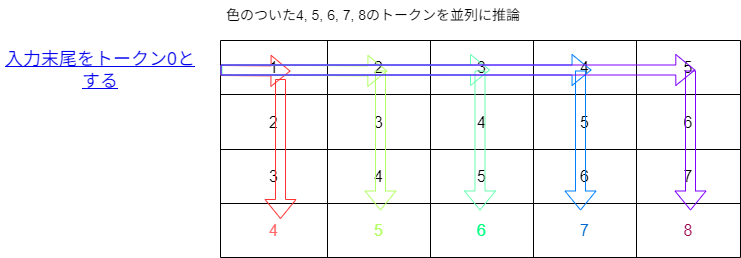
\includegraphics[width=0.8\textwidth]{img/lookahead_decoding/lookahead_branch.drawio.png}
  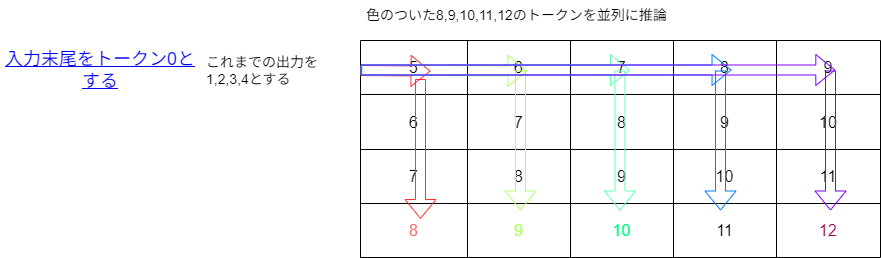
\includegraphics[width=0.8\textwidth]{img/lookahead_decoding/lookahead_branch2.drawio.png}
  \caption{Lookahead branchの概要図、$N = 4, W = 5$でのウィンドウ$W$の様子を表す、上の図は初めの状態、下の図は途中まで出力が決まった状態でのウィンドウの様子を示している。}
  \label{fig:lookahead_branch}
\end{figure}

\begin{figure}
  \centering
  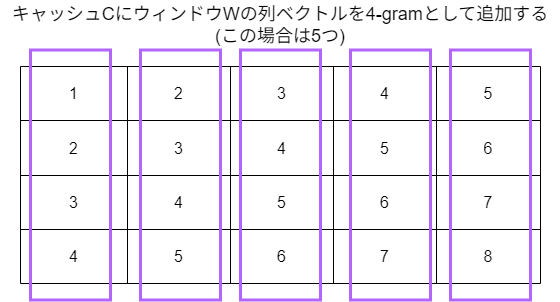
\includegraphics[width=0.8\textwidth]{img/lookahead_decoding/insert_cache.drawio.png}
  \caption{Lookahead branchで得られた候補をキャッシュ$C$に追加する様子。}
  \label{fig:insert_cache}
\end{figure}

上の四つのフェーズの説明は\url{https://github.com/hao-ai-lab/LookaheadDecoding?tab=readme-ov-file#lookahead-decoding-make-jacobi-decoding-feasible}のGIFがわかりやすい。
上の4つのフェーズを繰り返すことで、最終的な出力をアウトプットする。

その他の詳細について
\begin{itemize}
  \item VerificationはSample Verificationでより効率的に行える。
  \item Lookahead branchの推論は並列化可能である。
  \item またLookahead branch, Verification branchはそれぞれ独立に計算できるのも強み。
  \item FlashAttentionを用いることで、メモリI/Oを高速にできる。
\end{itemize}

\section{実験}

\subsection{モデル}
以下モデルの$7B, 13B, 34B, 70B$サイズを用いた。
\begin{itemize}
  \item LLaMA-2
  \item CodeLlama 
\end{itemize}

\subsection{データセット}
\begin{itemize}
  \item MT-bench: LLMの応答を評価するためのベンチマーク。
  \item GSM8K: 数学の問題を解くためのベンチマーク。
  \item HumanEval: コード補完のためのベンチマーク。
  \item MBPP: 命令ベースのコード生成。
  \item ClassEval: クラスレベルのコード補完。
\end{itemize}

\subsection{結果}
モデルベースラインとしてはHugging faceのGreedy searchでのデコーディング
を用いた。

\begin{itemize}
  \item 図\ref{fig:throughput_comparison}では、Lookahead decodingを使うことで少なくとも1.4倍程度高速化していることがわかる。
  \item 図\ref{fig:throughput_comparison_with_flash}では、FlashAttentionを用いることでさらに$20\%$ほど高速化されていることがわかる。
  \item 出力は元のものとは異なるため、出力の質が変化していないかどうかを確認した。
\end{itemize}

\begin{figure}
  \centering
  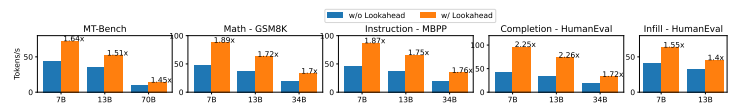
\includegraphics[width=\textwidth]{img/lookahead_decoding/fig5.png}
  \caption{Lookahead decodingのスループットのさまざまなデータセットでの比較}
  \label{fig:throughput_comparison}
\end{figure}

\begin{figure}
  \centering
  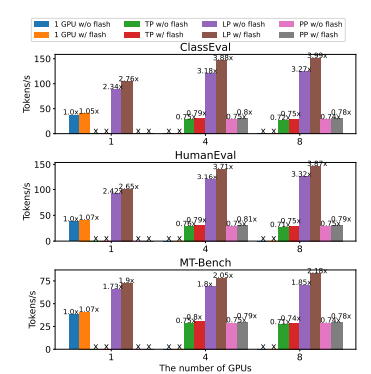
\includegraphics[width=0.5\textwidth]{img/lookahead_decoding/fig6.png}
  \caption{FlashAttentionを用いたときのLookahead decodingのスループットのさまざまなデータセットでの比較}
  \label{fig:throughput_comparison_with_flash}
\end{figure}

\section{感想}
\begin{itemize}
  \item 実装できるほどの解像度までは理解しきれていないが、かなり多くの部分が並列化できるようになっていて高速化できそうだし、実験結果でもそれが示されていて面白い。
  \item githubのREADMEにあるGIFと論文のアルゴリズムを照らしながら読まないと難しかった。
\end{itemize}

\bibliographystyle{jplain}
\bibliography{template.bib}

\end{document}